\documentclass[
    12pt, % Schriftgröße
    DIV10,
    ngerman, % für Umlaute, Silbentrennung etc.
    a4paper, % Papierformat
    oneside, % einseitiges Dokument
    titlepage, % es wird eine Titelseite verwendet
    parskip=half, % Abstand zwischen Absätzen (halbe Zeile)
    headings=normal, % Größe der Überschriften verkleinern
    listof=totoc, % Verzeichnisse im Inhaltsverzeichnis aufführen
    bibliography=totoc, % Literaturverzeichnis im Inhaltsverzeichnis aufführen
    index=totoc, % Index im Inhaltsverzeichnis aufführen
    captions=tableheading, % Beschriftung von Tabellen unterhalb ausgeben
    final % Status des Dokuments (final/draft)
]{scrartcl}

% Pakete

% Schrift ----------------------------------------------------------------------
\usepackage{lmodern} % bessere Fonts

% Paket für Kopfzeilen und Fußzeilen
\usepackage[
    automark, % Kapitelangaben in Kopfzeile automatisch erstellen
    headsepline, % Trennlinie unter Kopfzeile
    ilines % Trennlinie linksbündig ausrichten
]{scrpage2}

% Anpassung an Landessprache
\usepackage[ngerman]{babel}

% Umlaute ----------------------------------------------------------------------
%   Umlaute/Sonderzeichen wie äöüß direkt im Quelltext verwenden (CodePage).
%   Erlaubt automatische Trennung von Worten mit Umlauten.
% ------------------------------------------------------------------------------
\usepackage[utf8]{inputenc}
\usepackage[T1]{fontenc}
\usepackage{textcomp} % Euro-Zeichen etc.

\usepackage[babel,german=quotes]{csquotes}

% Bei Änderungen müssen die *.aux und *.bbl Dateien manuell gelöscht werden
% Sonst kommt es zu einem Fehler bei der Erstellung
%\usepackage[round, sort, comma, numbers]{natbib}
%\usepackage[round, numbers]{natbib}
%\bibliographystyle{abbrvdin}
%

\usepackage{scrhack}

\usepackage[citestyle=alphabetic,bibstyle=alphabetic,backend=biber]{biblatex}
\bibliography{Bibliographie}
\DefineBibliographyStrings{german}{
  bibliography = {Literaturverzeichnis},
}
\setlength\bibitemsep{8pt}

\usepackage{xpatch}
\xpretobibmacro{author}{\mkbibbold\bgroup}{}{}
\xapptobibmacro{author}{\egroup}{}{}
\xpretobibmacro{editor}{\mkbibbold\bgroup}{}{}
\xapptobibmacro{editor}{\egroup}{}{}
\xpretobibmacro{editor+others}{\mkbibbold\bgroup}{}{}
\xapptobibmacro{editor+others}{\egroup}{}{}
\xpretobibmacro{bbx:editor}{\mkbibbold\bgroup}{}{}
\xapptobibmacro{bbx:editor}{\egroup}{}{}

% Grafiken ---------------------------------------------------------------------
% Einbinden von JPG-Grafiken ermöglichen
\usepackage[dvips,final]{graphicx}
\graphicspath{{Bilder/}}

% Paket zur Verwendung zusätzlicher Positionsbefehle
\usepackage{float}

% Befehle aus AMSTeX für mathematische Symbole z. B. \boldsymbol \mathbb --------
\usepackage{amsmath,amsfonts}

% Einfache Definition der Zeilenabstände und Seitenränder etc. -----------------
\usepackage{setspace}
\usepackage{geometry}

% zum Umfließen von Bildern ----------------------------------------------------
\usepackage{floatflt}

% Farbdefinitionen
\usepackage{xcolor} 
\definecolor{hellgelb}{rgb}{1,1,0.9}
\definecolor{colKeys}{rgb}{0,0,1}
\definecolor{colIdentifier}{rgb}{0,0,0}
\definecolor{colComments}{rgb}{1,0,0}
\definecolor{colString}{rgb}{0,0.5,0}
\definecolor{whgreen}{RGB}{113,177,41}
\definecolor{dvBlue}{RGB}{0,85,160}

% URL verlinken, lange URLs umbrechen etc. -------------------------------------
\usepackage{url}

% PDF-Optionen -----------------------------------------------------------------
\usepackage[
    bookmarks,
    bookmarksopen=true,
    colorlinks=true,
% diese Farbdefinitionen zeichnen Links im PDF farblich aus
    linkcolor=dvBlue, % einfache interne Verkn�pfungen
    anchorcolor=black,% Ankertext
    citecolor=dvBlue, % Verweise auf Literaturverzeichniseintr�ge im Text
    filecolor=magenta, % Verkn�pfungen, die lokale Dateien �ffnen
    menucolor=dvBlue, % Acrobat-Men�punkte
    urlcolor=dvBlue, 
% diese Farbdefinitionen sollten für den Druck verwendet werden (alles schwarz)
%    linkcolor=black, % einfache interne Verkn�pfungen
%    anchorcolor=black, % Ankertext
%    citecolor=black, % Verweise auf Literaturverzeichniseintr�ge im Text
%    filecolor=black, % Verkn�pfungen, die lokale Dateien �ffnen
%    menucolor=black, % Acrobat-Men�punkte
%    urlcolor=black, 
    %backref, % Inkompatibel mit BibLateX
    plainpages=false, % zur korrekten Erstellung der Bookmarks
    pdfpagelabels, % zur korrekten Erstellung der Bookmarks
    hypertexnames=false, % zur korrekten Erstellung der Bookmarks
    linktocpage % Seitenzahlen anstatt Text im Inhaltsverzeichnis verlinken
]{hyperref}

% fortlaufendes Durchnummerieren der Fußnoten ----------------------------------
\usepackage{chngcntr}
%\counterwithout{footnote}{chapter}

% Formatierung von Listen ändern -----------------------------------------------
\usepackage{paralist} % itemize, enumerate

% bei der Definition eigener Befehle benötigt
\usepackage{ifthen} % Vielleicht nicht nötig

% definiert u.a. die Befehle \ und \listoftodos
\usepackage{todonotes}
\reversemarginpar

% sorgt dafür, dass Leerzeichen hinter parameterlosen Makros nicht als Makroendezeichen interpretiert werden
\usepackage{xspace}

\usepackage{tabularx} % Tabellenspalten mit variabler Breite
\usepackage{wrapfig}  % Schriftumflossene Bilder


% Seitenstil

% Zeilenabstand 1,5 Zeilen
\onehalfspacing

% Seitenränder
% bottom is 20 + X, weil Footer nicht berücksichtigt wird
\geometry{paper=a4paper,left=30mm,right=20mm,top=20mm, bottom=38mm, footskip=8mm}

% Kopf- und Fußzeilen ----------------------------------------------------------
% Kopf- und Fußzeile auch auf Kapitelanfangsseiten
%\renewcommand*{\chapterpagestyle}{scrheadings} 
% Schriftform der Kopfzeile
%\renewcommand{\headfont}{\normalfont}

% Kopfzeile
\ihead{\headmark} % links
\chead{}
\ohead{
\includegraphics[scale=0.1]{Bilder/DJLogo.png}} % rechts
\setlength{\headheight}{20mm} % Höhe der Kopfzeile
% Kopfzeile über den Text hinaus verbreitern
%\setheadwidth[0pt]{textwithmarginpar} 
\setheadsepline[text]{0.4pt} % Trennlinie unter Kopfzeile

% Fußzeile
%\ifoot{} % links
\cfoot{} % mitte
\ofoot{\pagemark} % rechts
%\setfootsepline[text]{0.4pt} % Trennlinie unter Kopfzeile



% Schusterjungen und Hurenkinder vermeiden
%\clubpenalty = 10000
%\widowpenalty = 10000 
%\displaywidowpenalty = 10000

% Verringert den Abstand über den Überschriften
%\renewcommand*{\chapterheadstartvskip}{\vspace*{-\topskip}}

% Irgendwas mit Silbentrennung in MonoSpace (texttt)
\newcommand{\origttfamily}{}% sollte noch nicht definiert sein!
\let\origttfamily=\ttfamily % alte Definition von \ttfamily sichern
\renewcommand{\ttfamily}{\origttfamily \hyphenchar\font=`\-}


% Eigene Befehle und typographische Auszeichnungen für diese

\newcommand{\bs}{$\backslash$}

% einige Befehle zum Zitieren --------------------------------------------------
\newcommand{\Zitat}[2][\
empty]{\ifthenelse{\equal{#1}{\empty}}{\citep{#2}}{\citep[#1]{#2}}}

% zum Ausgeben von Autoren
\newcommand{\AutorName}[1]{\textsc{#1}}
\newcommand{\Autor}[1]{\AutorName{\citeauthor{#1}}}

% Produktnamen
\newcommand{\produkt}[1]{\textbf{#1}}

\newcommand{\code}[1]{\texttt{#1}}

% zum Einbinden von Programmcode -----------------------------------------------
\usepackage{listings}
\usepackage{xcolor}
\usepackage{textcomp}
\lstset{
    float=hbp,
    basicstyle=\ttfamily\color{black}\small,
    identifierstyle=\color{colIdentifier},
    keywordstyle=\color{colKeys},
    stringstyle=\color{colString},
    commentstyle=\color{colComments},
    columns=flexible,
    tabsize=2,
    frame=single,
    extendedchars=true,
    showspaces=false,
    showstringspaces=false,
    numbers=left,
    numberstyle=\ttfamily\small,
    numbersep=5pt,
    breaklines=true,
    backgroundcolor=\color{hellgelb},
    breakautoindent=true
}

\lstset{literate=
  {á}{{\'a}}1 {é}{{\'e}}1 {í}{{\'i}}1 {ó}{{\'o}}1 {ú}{{\'u}}1
  {Á}{{\'A}}1 {É}{{\'E}}1 {Í}{{\'I}}1 {Ó}{{\'O}}1 {Ú}{{\'U}}1
  {à}{{\`a}}1 {è}{{\'e}}1 {ì}{{\`i}}1 {ò}{{\`o}}1 {ù}{{\`u}}1
  {À}{{\`A}}1 {È}{{\'E}}1 {Ì}{{\`I}}1 {Ò}{{\`O}}1 {Ù}{{\`U}}1
  {ä}{{\"a}}1 {ë}{{\"e}}1 {ï}{{\"i}}1 {ö}{{\"o}}1 {ü}{{\"u}}1
  {Ä}{{\"A}}1 {Ë}{{\"E}}1 {Ï}{{\"I}}1 {Ö}{{\"O}}1 {Ü}{{\"U}}1
  {â}{{\^a}}1 {ê}{{\^e}}1 {î}{{\^i}}1 {ô}{{\^o}}1 {û}{{\^u}}1
  {Â}{{\^A}}1 {Ê}{{\^E}}1 {Î}{{\^I}}1 {Ô}{{\^O}}1 {Û}{{\^U}}1
  {œ}{{\oe}}1 {Œ}{{\OE}}1 {æ}{{\ae}}1 {Æ}{{\AE}}1 {ß}{{\ss}}1
  {ç}{{\c c}}1 {Ç}{{\c C}}1 {ø}{{\o}}1 {å}{{\r a}}1 {Å}{{\r A}}1
  {€}{{\EUR}}1 {£}{{\pounds}}1
}

\usepackage{microtype}

\renewcommand*{\dictumwidth}{.41\textwidth}
\renewcommand*{\dictumrule}{}
\renewcommand*{\dictumauthorformat}[1]{--- #1}
\setkomafont{dictumauthor}{%
\scshape
}

\definecolor{bluekeywords}{rgb}{0,0,1}
\definecolor{greencomments}{rgb}{0,0.5,0}
\definecolor{redstrings}{rgb}{0.64,0.08,0.08}
\definecolor{xmlcomments}{rgb}{0.5,0.5,0.5}
\definecolor{types}{rgb}{0.17,0.57,0.68}

\lstdefinestyle{csharp}
{
    language=[Sharp]C,
    captionpos=b,
    %numbers=left, %Nummerierung
    %numberstyle=\tiny, % kleine Zeilennummern
    showspaces=false,
    showtabs=false,
    breaklines=true,
    showstringspaces=false,
    breakatwhitespace=true,
    escapeinside={(*@}{@*)},
    commentstyle=\color{greencomments},
    morekeywords={partial, var, value, get, set},
    keywordstyle=\color{bluekeywords},
    stringstyle=\color{redstrings},
    basicstyle=\ttfamily\small,
}

\lstdefinestyle{xml}
{
    language=XML,
    captionpos=b,
    %numbers=left, %Nummerierung
    %numberstyle=\tiny, % kleine Zeilennummern
    showspaces=false,
    showtabs=false,
    breaklines=true,
    showstringspaces=false,
    breakatwhitespace=true,
    escapeinside={(*@}{@*)},
    commentstyle=\color{greencomments},
    morekeywords={encoding},
    keywordstyle=\color{bluekeywords},
    stringstyle=\color{redstrings},
    basicstyle=\ttfamily\small,
}

\usepackage{wasysym}
\usepackage{ upgreek }

%\usepackage{caption} 
%\captionsetup[table]{skip=100pt}
% Bindet die Literaturdaten ein!
\bibliography{Bibliographie}
\begin{document}

%Startstruktur
\setcounter{secnumdepth}{3}
\setcounter{tocdepth}{3}

\pagestyle{empty}
\thispagestyle{plain}
\begin{titlepage}

\begin{center}


\includegraphics[scale=0.7]{Deckblatt/WH_Logo.jpg}

\vspace{2cm}

\Huge{\textbf{Drunken-Jukebox}}\\[1.5ex]
\Large{\textbf{Projektdokumentation}}
\rule{\textwidth}{0.4pt}\\[3.0ex]

\large{\textbf{im Masterstudiengang Verteilte Systeme}}\\[3.0ex]

\normalsize
\begin{tabular}{ll}\\
	vorgelegt von: 
	& \quad Daniel Hardes, Dennis Miller, \\[1.2ex]
	& \quad Fabian Paus, Christian Schlütter\\[1.2ex]
	& \quad \\[1.2ex]
	Modul:  & \quad Middleware A (MWA) \\[1.2ex]
	Gutachter:  & \quad Prof. Dr. Martin Guddat \\[1.2ex]
	Abgabetermin:  & \quad \today\\[1.2ex]
\end{tabular}

\end{center}

\end{titlepage}


\tableofcontents
\setcounter{page}{1}

\pagestyle{scrheadings}

\newpage

\section{Einleitung}
Im Rahmen des Moduls Middleware A im vergangenen Semester hatten wir die Idee der Drunken-Jukebox. Dabei handelt es sich um ein System zur automatisierten Musikgestaltung auf einer Party, bei der die Gäste durch Voten von Songs die Musik-Playlist und damit den als nächstes gespielten Song beeinflussen können. Nachdem im Modul Middleware A ein entsprechendes Backend entwickelt worden ist, besteht die Aufgabe im Modul Middleware B nun daraus entsprechende Client-Applikationen unter Benutzung des Google Web Toolkits zu entwickeln. 

Entsprechend der Idee aus Middleware A soll es drei Client-Applikationen geben, die es zu realisieren gilt. Wir beschränken uns in diesem Projekt auf die Anwendungen für den Administrator und für den Partygast. Die dritte Anwendung zum Abspielen der Musik, haben wir bereits rudimentär in der Veranstaltung Middleware A implementiert. Aufgrund diverser fortwährender Probleme mit dem Applikationsserver WildFly, werden die Anwendungen im Rahmen dieses Projekts auf Deployd \footnote{\url{http://deployd.com/}} als alternatives Backend zugreifen. Im Nachfolgenden wird dieses wie auch die Planung, das Design sowie die letztendliche Realisierung der Client-Anwendungen vorgestellt. Es galt möglichst viele verschiedene Facetten, dessen was in GWT möglich ist, zu nutzen.

\section{Anforderungen}

2 Anwendungen

\subsection{Admin}
- Verwaltung von
  - Songs
  - Party
  
Mockups einfügen und Funktionen erklären

\subsection{Vote-App}
- Anzeige der aktuellen Playlist (Send DI fehlt im Mockup)
- Voten
- DI (Mockup fehlt)

Mockups einfügen und Funktionen erklären

Chris
\section{Realisierung}

In diesem Kapitel wird die konkrete Umsetzung der Anforderungen in GWT beschreiben.
Zuerst wird die Architektur der Anwendung festgelegt. Anschließend werden konkrete
Implentierungsdetails erläutert, welche die Erstellung eigener Widgets in GWT und
mittels JSNI, das Styling in GSS sowie die Lokalisierung umfassen.

\subsection{Architektur}

Um den Anforderungen der zwei Anwendergruppen (Veranstalter und Gäste einer Party) gerecht
zu werden, entwickeln wir zwei Anwendungen. Die Admin-Oberfläche wird als Desktop-Webanwendung
entwickelt, während die Vote-App als mobile Webanwendung umgesetzt wird. Trotzdem werden
beide Anwendungen mit einer ähnlichen Softwarearchitektur implementiert.

\begin{figure}[tbh]
\centering
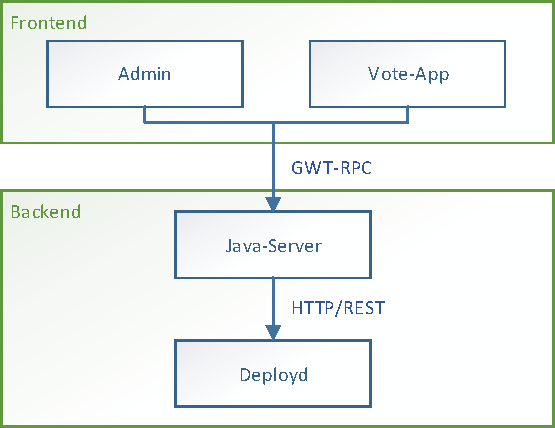
\includegraphics[width=0.7\linewidth]{Bilder/Architektur-Ueberblick}
\caption{Überblick über die Architektur der beiden Anwendungen}
\label{fig:Architektur-Ueberblick}
\end{figure}

\subsubsection{Frontend}
MVP-Architektur
- Klassendiagramm für beide (Views \& Presenter)

\subsubsection{Backend}
- Java-Server
- Als Proxy für Deployed
- Deployed zur Datenhaltung + Logik

Fabian

\subsection{Eigene Widgets}
- Search Dinge
- PlaylistEntries

Beispiele

Chris

\subsection{Styles in GSS}
Für das Styling der beiden GWT-Anwendungen verwenden wir GSS. Da es unterschiedliche Anforderungen
an Deskop- und Mobilanwendungen gibt, werden zwei Stylesheet-Dateien verwendet.

- Verknüpfung: Client-Bundle und GSS-Dateien
- Gemeinsame Styles auslagern?

Fabian

\subsection{Lokalisierung}
Beide Anwendungen sollen lokalisiert in Deutsch und Englisch angeboten werden.
Im Admin soll es möglich sein die Sprache über die Oberfläche zu ändern, während
in der Vote-App die Sprache automatisch ausgewählt wird.

Dazu verwenden wir Ressourcen-Strings (TODO).

Fabian

\subsection{JSNI}
Slider mit jQuery

Daniel
\newpage
\section{Fazit}
Aus dem Projekt heraus ist eine Anwendung entstanden, in der die Projektidee realisiert wurde. Unter Verwendung des Anwendungsservers WildFly haben wir das Backend für die Drunken-Jukebox implementiert.
Basierend auf dem Datenmodell, das wir zu Beginn des Projekts, persistiert der Anwendungsserver entsprechende Daten in einer frei wählbaren Datenbank. Die Anwendungslogik befindet sich in den Sessionbeans, welche innerhalb der externen Schnittstellen verwendet werden. So haben wir die Event-Subscribe-Methodik anhand eines Topics umgesetzt und eine REST-Schnittstelle geschaffen, die benötigte Beans injectet. Mittels dieser Schnittstellen ist das Backend bestens für den Einsatz vorbereitet. 

Rückblickend auf das gesamte Projekt stellen wir fest, dass wir zu Beginn hohe Erwartungen an den Applikationsserver gehegt haben und von dessen konzeptioneller Idee begeistert waren. Leider entwickelte sich unser Gesamteindruck des Produktes WildFly während des Praxiseinsatzes gegenteilig. 
Die Anbindung unterschiedlicher Datenbankmanagementsysteme funktionierte erwartungsgemäß gut. Unser Datenmodell lies sich dabei problemlos abbilden. Im darauf folgenden Schritt schwand unsere Zuversicht schon bei dem Versuch Beans in einem REST-Service zu injecten. Erst nach einer Änderung unserer Architektur ließen sich dieses und kleinere weitere Probleme lösen. Ebenfalls verlief der Einsatz des Konzepts zur Authentifizierung und Autorisierung alles andere als zufriedenstellend, so dass auch mit Abschluss dieses Projekts das Konzept noch nicht vollständig für alle Bereiche (Beans, Webservice und Topics) funktioniert.
Diese elementaren Probleme in Kombination mit Fehlermeldungen, die meist keine Aussagekraft besitzen, und einer mangelhaften Dokumentation des Applikationsserver WildFly haben unseren Gesamteindruck zusätzlich negativ geprägt. Trotz des umfangreichen Engagements aller Projektbeteiligten konnten nicht alle Probleme beseitigt werden.

In einem kurzen Ausblick lässt sich festhalten, dass zu aller erst einmal die noch vorhandenen Probleme rund um die Authentifizierung bzgl. des Topics gelöst werden müssen, damit das Backend einsatzfähig ist. In weiteren Schritten sollten die Anwendungen für die Endanwender entwickelt werden. So gilt es eine Smartphone-App für die Party-People und ein Webinterface für den Admin bzw. den DJ zu entwickeln. Darüber hinaus muss ein Player zum Abspielen der Musik entwickelt werden, der mit der laufenden Anwendung auf dem Applikationsserver kommuniziert.
Sind die aufgezählten Anwendungen ebenfalls entwickelt, beginnt die Testphase. Eine mögliche Idee wäre der erstmalige Test auf einer Veranstaltung der Hochschule. Sind alle elementaren Funktionen erfolgreich implementiert, lassen sich weitere Features umsetzen.

\appendix
\section{GWT-RPC}

\subsection{Admin Service}
Nachfolgend eine Liste aller Funktionen des Admin-Services:
\begin{description}
	\item[ArrayList<Song> getSongList()] Gibt die Liste aller Songs zurück.
	\item[Song getSong(String id)] Gibt einen spezifischen Song zurück.
	\item[Song updateSong(Song song)] Updatet einen Song.
	\item[void removeSong(String songId)]	Löscht einen Song.
	\item[Song addSong(Song song)] Fügt einen neuen Song hinzu.
	\item[Party startParty()]	Startet eine Party
	\item[Party stoppParty(Party p)] Stoppt eine Party
	\item[GlobalPlaylist getPlaylist()] Gibt die aktuelle Playlist zurück zurück.
\end{description}


\subsection{VoteApp Service}
Nachfolgend die Auflistung der Funktionen des VoteApp-Services:
\begin{description}
	\item[Song getCurrentSong()] Gibt den Current Song zurück.
	\item[PlayList getPlayList()]	Gibt die aktuelle Playlist zurück.
	\item[void sendDi(int value)] Sendet den übergebenen Betrunkenheitsgrad (DI-Wert) zurück.
	\item[void sendVote(PlayListEntry entry, Vote vote)] Sendet zum Übergebenen Song (PlaylistEntry) einen Vote (UP oder DOWN).
\end{description}

\section{REST-Schnittstelle von Deployd}

\subsection{party}
\label{service:party}
Erstellt eine neue Party und löscht die playlist.

POST
\url{/party}

Parameter: Leeres JSON Objekt

Rückgabewert: JSON Objekt der Party
Beispiel:
\begin{lstlisting}
{
"start":"2015-06-03T12:12:48.190Z",
"end":{},
"avgDI":0,
"guestCount":1,
"id":"791bbdf86d85fa29"
}
\end{lstlisting}

\subsection{playlist}
\label{service:playlist}
Gibt die aktuelle Playlist zurück.

GET
\url{/playlist}

Rückgabewert: JSON Array aller Playlist Einträge
Beispiel:
\begin{lstlisting}
[
{"songID":"89d0ddbf0d7e683e","position":0,"votes":1,"id":"b90bb3e138456920"},
{"songID":"fbc56a0eacd2d880","position":0,"votes":2,"id":"7de1eb1dfeee188e"},
...
]
\end{lstlisting}


\subsection{currentSong}
\label{service:currentSong}
Gibt den current Song zurück.

GET
\url{/currentsong}

Rückgabewert: JSON Objekt des current Songs
Beispiel:
\begin{lstlisting}
[{
"songID":"18c77e30e376280f",
"id":"77a26abb92f2ebdd"
}]
\end{lstlisting}

\subsection{song}
\label{service:song}
Gibt alle Songs zurück.

GET
\url{/song}

Rückgabewert: JSON Array aller Songs
Beispiel:
\begin{lstlisting}
[{
"title":"The Pretender",
"length":260,
"artist":"Foo Fighters",
"source":"C:\\Musik\\",
"sourceType":0,
"genres":"Rock",
"id":"89d0ddbf0d7e683e"
},
{"title":"Crawling",
"length":340,
"artist":"Linkin Park",
"source":"C:\\Musik\\",
"sourceType":0,
"genres":"Rock",
"id":"fbc56a0eacd2d880"
},
...
]
\end{lstlisting}



Zudem wir noch POST, PUT, und DELETE unterstützt\footnote{\url{http://docs.deployd.com/docs/collections/reference/http.html}}.




\newpage
%\printbibliography

\end{document}